\documentclass[../template]{subfiles}

\begin{document}
\section{Minimum Spanning Tree}

\begin{center}
    \begin{tikzpicture}[rotate=90]
        \Vertices[unit=2.3]{circle}{A,B,C,D,E}
        %\Edges(A,B,C,D,E)
        \Edge[color=red, label=$10$](A)(C)
        \Edge[label=$8$](A)(D)
        \Edge[color=red, label=$7$](D)(E)
        \Edge[color=red, label=$4$](A)(E)
        \Edge[color=red, label=$3$](B)(A)
        \Edge[label=$9$](B)(D)
        \Edge[label=$5$](B)(E)
        ;
    \end{tikzpicture}
\end{center}
\subsection{Algoritmo di Kruskal (Greedy)}
\lstinputlisting{algorithms/mst_kruskal.py}
\subsection{Correttezza algoritmo di Kruskal}
Supponiamo per assurdo che esista un' diverso MST $T' = (V,E_{T'})$ di peso inferiore a $T = (V, E_T)$,
quello restituito dall'algoritmo greedy.

Siccome i due alberi hanno costo diverso, differiscono di almeno un' arco.
Indichiamo con $e_h$ l'arco a peso minore appartenente a $\{E_T - E_{T'}\}$.
Dato che $T'$ è un MST, esiste un ciclo $C$ in $\{e_h\} \cup E_{T'}$ contenente l'arco $e_h$.
Siccome anche $T$ è un albero, quindi non ha cicli, allora $C \cap E_{T} \neq \emptyset$.
Chiamiamo $e_r$ l'arco a peso minore appartenente a $C \cap \{E_{T} - E_{T'}\}$.
Necessariamente $w_{e_r} \le w_{e_h}$, altrimenti l'algoritmo greedy applicato a $T$ avrebbe selezionato prima $e_h$ al posto di $e_r$.
Sostituendo in $T'$ l'arco $e_r$ con $e_h$ ottengo un nuovo albero di peso inferiore.

Questo va contro l'ipotesi $T'$ è l'albero di supporto a peso minore.
\subsection{Analisi complessità algoritmo greedy}
$O(E \cdot \log (E))$, dovuta all'ordinamento degli archi in ordine di peso.
Il controllo dell'esistenza di cicli è effettuato in $O(1)$.

\subsection{Foresta di supporto}
Viene chiamata foresta di supporto di un grafo $G$ un grafo parziale $F = (V, E_F)$ privo di cicli. In particolare, un albero di
supporto è una foresta con una sola componente connessa.

\subsubsection{Teorema}
Indichiamo con $(V_1, E_1),\ldots ,(V_k, E_k)$ le componenti connesse di una foresta di supporto
$F = (V, E_F)$ del grafo $G$. Sia inoltre $(u, v)$ un arco a peso minimo tra quelli con un unico estremo
in $V_1$. Allora esiste almeno un albero di supporto a peso minimo appartenente a $\bigcup^k_{i=1} E_i$,
che contiene $(v, v)$.

\subsubsection{Dimostrazione}
Per assurdo, l'albero a peso minimo non contiene $(u, v)$. Ma aggiungendo $(u, v)$ a tale albero si forma un
ciclo contenente un altro arco $(u', v')$  con un solo estremo in $V_1$.
Se si toglie questo arco e si lascia $(u, v)$ si ottiene un albero di peso minore,
contraddicendo l'ipotesi.

\subsection{Algoritmo MST-1}
\begin{center}
    \begin{tikzpicture}[rotate=90]
        \Vertices[unit=2.3]{circle}{0,1,2,3,4}
        %\Edges(A,B,C,D,E)
        \Edge[color=red, label=$3$](0)(1)
        \Edge[label=$5$](0)(2)
        \Edge[label=$9$](0)(3)
        \Edge[label=$20$](0)(4)

        \Edge[color=red, label=$4$](1)(2)
        \Edge[label=$8$](1)(3)
        \Edge[color=red, label=$10$](1)(4)

        \Edge[label=$7$, color=red](2)(3)
        \Edge[label=$11$](2)(4)

        \Edge[label=$12$](3)(4)
        ;
    \end{tikzpicture}
\end{center}
\lstinputlisting{algorithms/mst_1.py}

\subsection{Correttezza MST-1}
\end{document}
